\subsection{Divider}
\label{sec:div}


The algorithm implemented in the original version of the processor is one of the simplest but the
slowest available: a radix-2 non restoring division.

Several other algorithms can compute the division faster but all of them present disadvantages
that must be taken into account according to the target application.

Algorithms like repeated multiplication or reciprocation are fast but require a significant amount
of area because they make use of a whole multiplier to work which in itself is quite a big circuit.
Similarly an array divider would have been very fast given we had control of the
place\&routing process in order to create a regular structure. However this is not possible in FPGAs so we discarded that option. 

For these reasons we decided to implement
a simple radix-4 division algorithm for simplicity of implementation and of the circuit itself.

Another possibility was to use an higher radix as this could have improved performance but the size of the lookup table required
by the algorithm would have increased the area consumption.
However the area itself is not a significant concern since, as stated previously, we are focused on power consumption and execution time. Notwithstanding a larger circuit means harder computations and thus more energy consumption.

The divider consist of a state machine (its diagram is shown in figure~\ref{fig:div_state_dia}) which checks if the inputs will
generate an overflow by doing a trial subtraction between the divisor and the MSBs of the dividend. Thereafter it performs a preliminary shift to put the divisor in the appropriate range in order to match the correct range for the look-up table to work properly.


\begin{figure}[H]
\centering
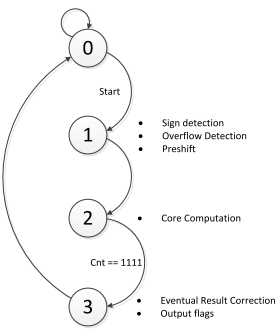
\includegraphics[width=0.85\textwidth,height=0.4\textheight,keepaspectratio]{DivisorStateMachine.png}
\caption{Divider State Diagram.}
\label{fig:div_state_dia}
\end{figure}

Figure~\ref{fig:div_state_dia} also shows when the ready signals are asserted. The documentation~\cite{doc} explains the ready signal must be set the cycle before the result is stable, thus in the last state of the state machine. The reason for this is that once the machine returns to the idle state the registers are ``frozen'' and the results is stable. The \texttt{nready} signal must be asserted 3 cycles before the results is stable. This cycle is reached when during the core computation the counter's value is 14 (``\texttt{1110}''). 
By observing these signals the integer unit can find out when the operation is finished in order to eventually fetch consequent instructions or to make the pipeline proceed one step further.

After that, the real computation begins and lasts 16 clock cycles. The block diagram of the divider
while it is in this state is shown in figure~\ref{fig:div_block_dia}.

\begin{figure}[H]
\centering
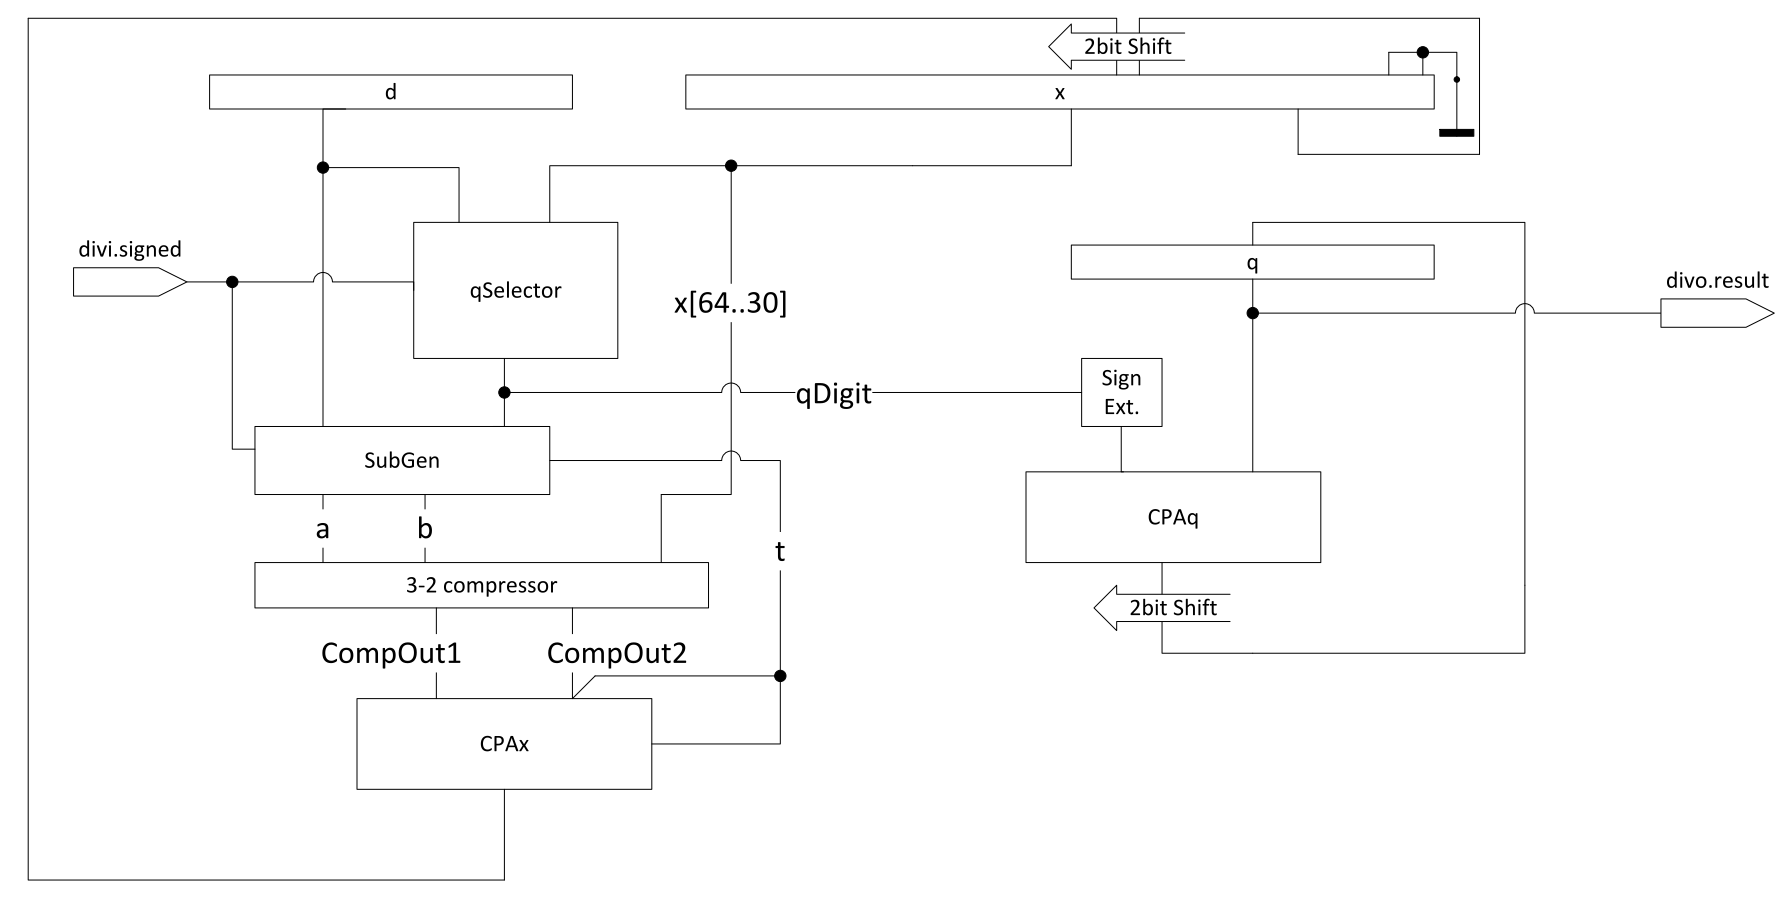
\includegraphics[width=1\textwidth,height=0.4\textheight,keepaspectratio]{DivisorDiagram.png}
\caption{Divider Block Diagram (during Core Computation, State = 1).}
\label{fig:div_block_dia}
\end{figure}

The algorithm is very similar to the original radix-2 version but in this case the partial reminder (x)
is shifted by 2 bits every cycle and the circuit has to guess the quotient digit from the range [-3,3].
``\texttt{qSelector}'' is the lookup table which performs the quotient digit guessing and it's based on the p-d
plot of the radix-4 SRT division shown in figure~\ref{fig:div_pd_plot}. In case of unsigned division only the right half of
the p-d plot is being used.

\begin{figure}[H]
\centering
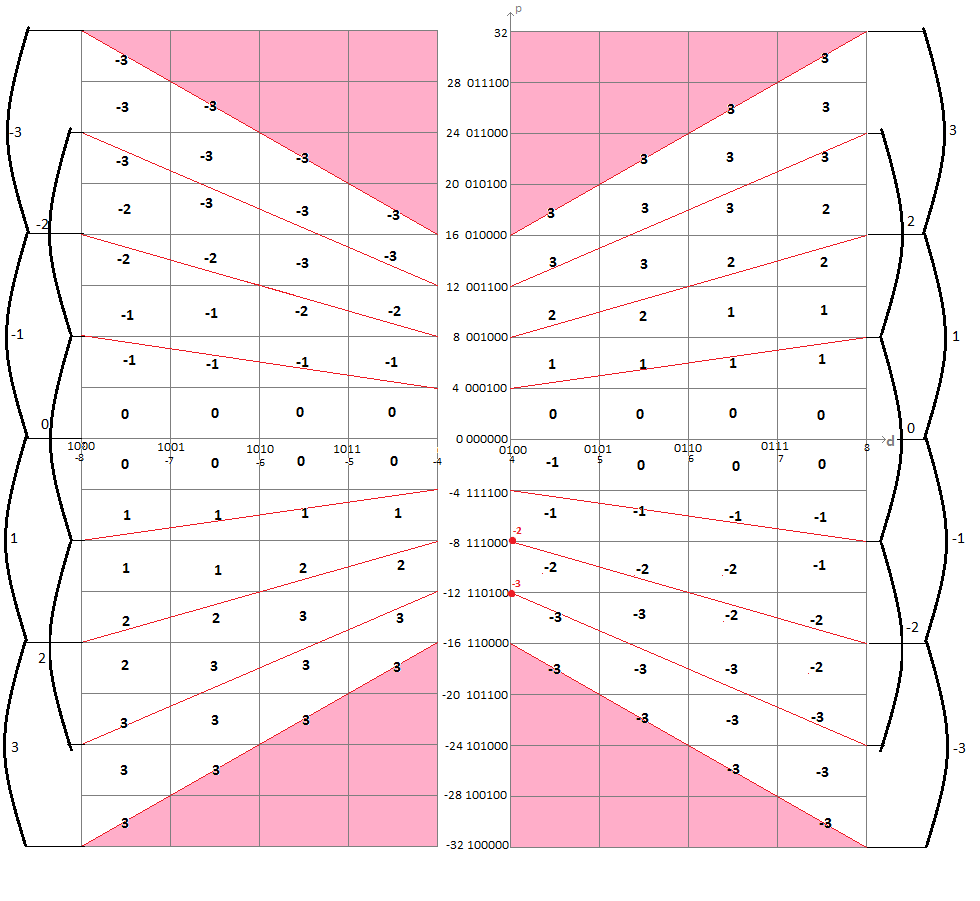
\includegraphics[width=0.85\textwidth,height=0.85\textheight,keepaspectratio]{radix4pd.png}
\caption{Radix-4 P-D Plot (Red Dots are Exceptions).}
\label{fig:div_pd_plot}
\end{figure}

The quotient digits are in a radix-4 redundant format so a conversion to binary format is needed.
The conversion is performed gradually every cycle by the 32-bit adder ``CPAq'' which shifts and sums
each generated digit with the already calculated quotient.

An addition/subtraction in Carry-Save format would have been much faster and also easier for both the quotient and the partial reminder, but the selection of the quotient digit would have required the analysis of the most significant bits of
both the sum and the carry of the reminder (x). This would make the lookup table several orders of magnitude larger and therefore consume more area.

In our divider ``SubGen'' generates the multiple of d to sum with the current partial reminder in a
carry save format. All these operands are reduced by a 3-2 compressor (1 full adder of
delay) and finally the new partial reminder is calculated with a 35-bit adder, ``CPAx''.

Using this architecture is possible to easily calculate the triples of d allowing us to have a simpler p-d plot and consequently a smaller look-up table. In particular the -3d, which is the most difficult, is calculated as the negation of 2d concatenated with a 1 plus the negation of d. The signal t is set to 1 so it can be summed twice in the compressor and as the carry input of CPAx. In this way its weight is 2 and calculation of the 2s complement of 2d is finished.

The principle behind the calculation of the multiples is explained better in figure~\ref{fig:div_subGen}.

\begin{figure}[H]
\centering
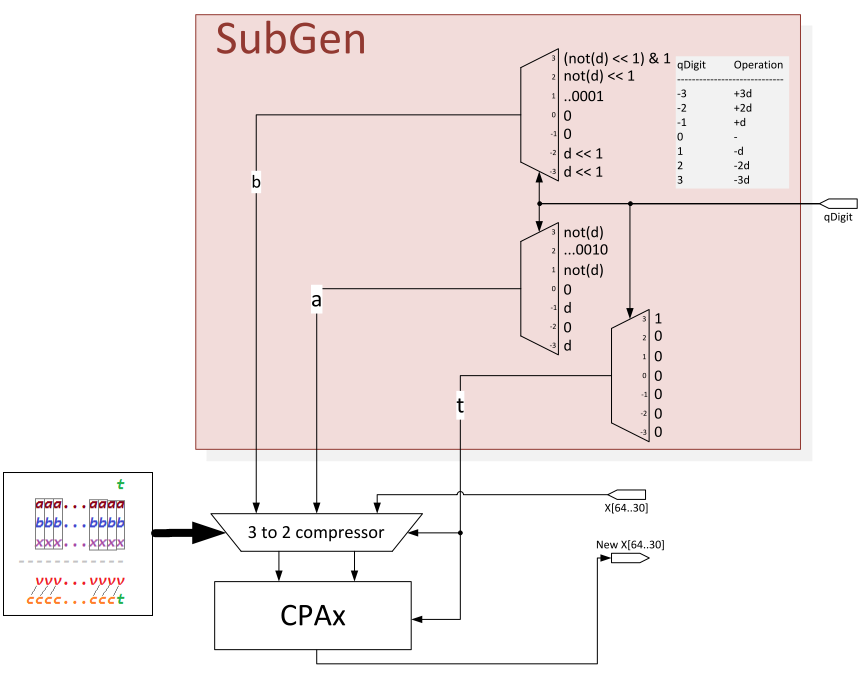
\includegraphics[width=1.5\textwidth,height=0.5\textheight,keepaspectratio]{SubGenExplanation.png}
\caption{Detail of SubGen (d multiples generator based of the qDigit).}
\label{fig:div_subGen}
\end{figure}

Other solutions have been analyzed, such as having a lookup table only for unsigned division, half
of the size of the final version, and handle the sign separately. But the synthesis has shown that the
resource utilization would have not changed significantly while one more cycle would have been needed.
Hence, we decided to keep the current divider.

At last, in order to check the compatibility of the radix-4 divider with the rest of the system, and its correct functioning, we designed a testbench.
In this testbench we placed both the old version and the new version of the divider and the inputs are routed to the two units equally, so we expect to have the same outputs in both but with different latencies.
Of course it's prohibitive to test the unit for all possible inputs therefore we determined a set of critical operations to test the design.

There are some categories of operations in this case, simple signed/unsigned division such as $350/100$ or -$350/100$ which can be performed with the signed signal asserted or not, operations involving exceptions in the p-d plot, and operations generating overflows.
The first category is not critical but just to be sure and have a complete testbench we implemented some of them.

As shown in figure~\ref{fig:div_pd_plot}, there are a couple of exceptions in the p-d plot. These exceptions are handled by the qSelector apart from all the other cases with dedicated lines of code (simple ifs).
For instance one of these exceptions is when the divisor is ``0100'' and the dividend is ``111000'' followed by zeros (otherwise it would not be an exception because the point would be inside the uncertanties area and not in the bottom left corner). In this scenario the quotient digit must be -2 instead of -1 so one of these operations could simply be -$16/4$ for this operation after the pre-shift the input of qSelector would be exactly these ones.

For the operations involving overflows there are several possibilities where the dividend is very high and the divisor very low, enough to make the result greater than $2^{32}$. There are also some operations that when considered to be signed don't generate overflows while if unsigned they do. This happen when the most significant bit of the dividend is one, its weight is $2^{63}$ when unsigned and -$2^{64}$ when signed and so it can change significantly the absolute value of the result.

All of the aforementioned operations have been analyzed in the appropriate testbench, whose simulation are partially shown in figure~\ref{fig:div32_wave}. The result is always the same as the baseline version of the divider. The only exception occurs when there is an overflow. Here the result of the radix-4 divider is different from the baseline, sometimes the simulator displays an ``X'' because in an overflow the qSelector works in some of the not allowed areas. Nonetheless the overflow flag is asserted normally so the processor won't consider the actual result and consequently this difference does not constitute a problem.

\begin{figure}[H]
\centering
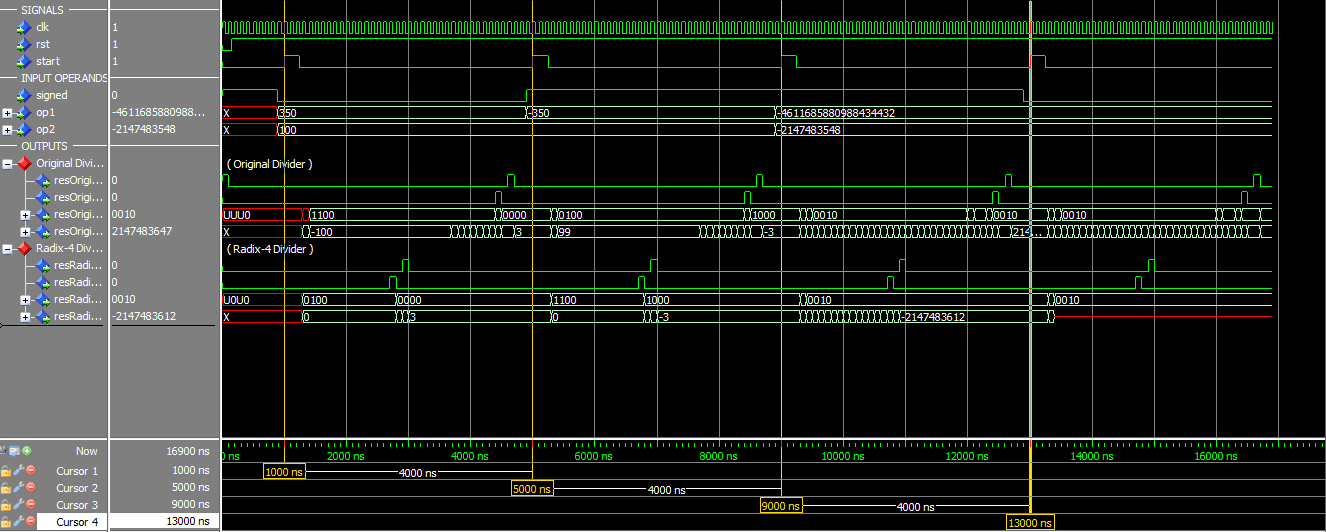
\includegraphics[width=1\textwidth,height=0.8\textheight,keepaspectratio]{myDivisionvsOriginal.png}
\caption{Signal Dump Of Radix-4 Divider Vs. Original Divider.}
\label{fig:div32_wave}
\end{figure}
